\documentclass[12pt]{article}
\usepackage{amsmath}
\usepackage{amssymb}
\usepackage{amsfonts}
\usepackage{array}
\usepackage{graphicx}% use this package if an eps figure is included.
\usepackage{mathrsfs}
\usepackage{multirow}
\usepackage{siunitx}
\setlength\topmargin{-1.1in} \addtolength\textheight{2.1in}
\addtolength{\oddsidemargin}{-0.2in}
\addtolength{\evensidemargin}{-0.1in} \textwidth 5.8in
\newcounter{questioncounter}
\newcounter{equestioncounter}
\setlength\parskip{10pt} \setlength\parindent{2em}

\begin{document}
\title{Gesture Based Turn Signaling System Proposal}

\author{Sultan Alnuaimi, Edan Elazar and Kaylan Wang\\
\small \{saltana2, eelazar2, kaylanw2\}@illinois.edu\\
\small University of Illinois Urbana-Champaign, ECE 445\\
\small TA: Sanjana Pingali}
\maketitle

% \begin{abstract}
% A temperature wave propagates along a long thin bar of a metallic sample when subjected to periodic heating. In this way it is demonstrated that there is no wave nature in these improperly called thermal waves by showing that they do not transport energy and its propagation properties can be used to determine the thermal diffusivity of the material.
% \end{abstract}

\section{Introduction}
\subsection{Problem}
Cyclists, skateboarders, and scooter riders often face 
challenges in signaling their intentions to drivers, 
especially in low-light conditions. The traditional
 method of using hand signals is not always visible or 
 practical, particularly at night or during adverse weather 
 conditions. This lack of clear communication can lead to 
 dangerous situations on the road, as other motorists may 
 fail to recognize the cyclist's intended maneuvers, or if 
 an accident occurs. 

\subsection{Solution}

To address this issue, we propose the development of a gesture 
recognition-based turn signaling system for cyclists and scooter 
riders. This system will utilize a combination of sensors, such 
as accelerometers and gyroscopes, integrated into a wearable 
like a jacket. Then we process the sensor data to identify 
specific arm gestures made by the rider and activate corresponding 
LED signals. For example, if the rider extends their arm straight 
to the left, the left turn signal is activated, or if the rider 
indicates a stop, then the brake light is activated, and so on. 
Additionally, the sensors will be able to detect when the rider 
has had an accident or a crash, and activate a hazard signal. 

We propose placing an IMU above (or below depending on how hard 
it is to differentiate between movements) the elbow on each arm 
of the wearable. The microprocessor will then receive and process 
the data from the IMU, determining what kind of movement has been 
made. Then, depending on the movement, it will output a specific 
signal to the LEDs to display on the back and arms of the wearable. 


\subsection{Visual Aid}
\begin{figure}[ht]
    \centering
    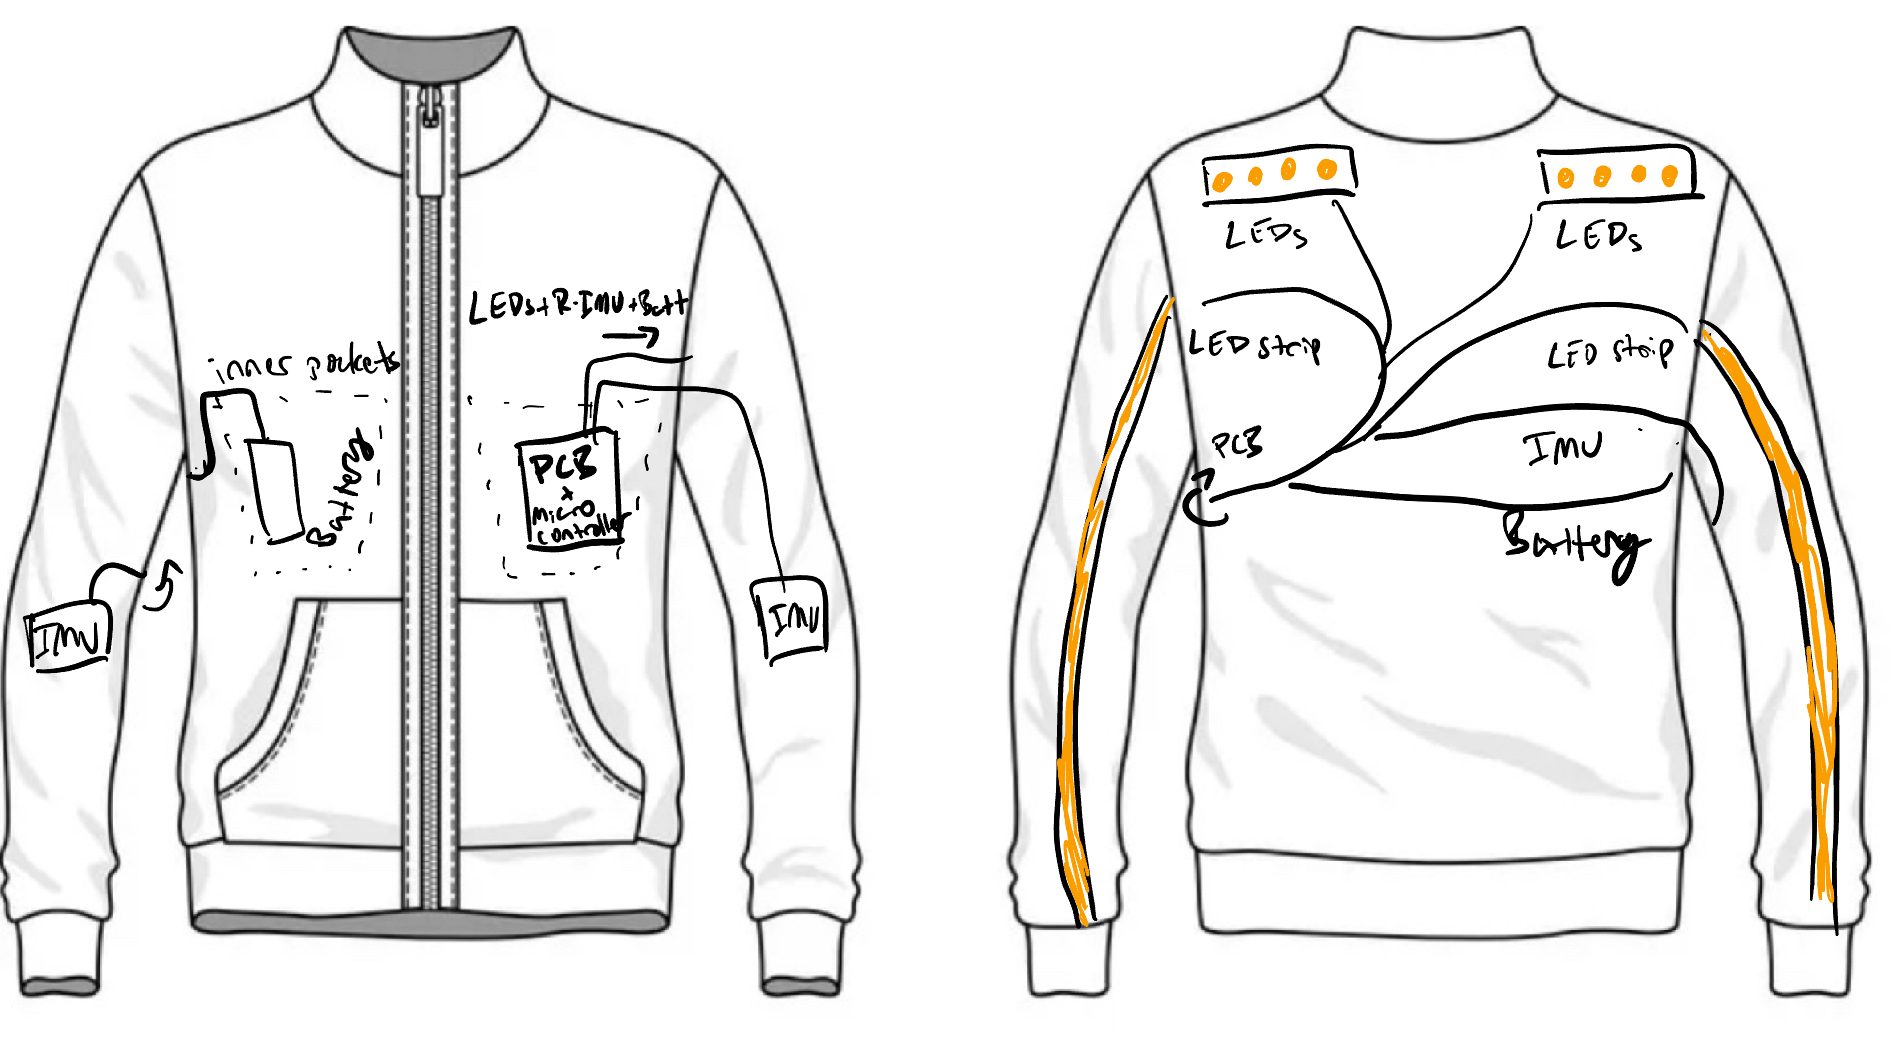
\includegraphics[width=0.8\textwidth]{visual_aid.jpeg}
    \caption{Visual Aid mockup of the wearable}
    \label{fig:my_label}
\end{figure}
\subsection{High Level Requirements}
\begin{enumerate}
    \item The device should be able to last at least 1 hour on a full battery.
    \item The device should correctly detect and interpret specific arm 
    gestures with a signal recognition accuracy of 90%. 
    \item The LEDs should be visible from a distance of at least 
    250 feet in low light conditions to ensure that they are clearly visible at both day and night. 
\end{enumerate}
\newpage
\section{Design}
\subsection{Block Diagram}
\begin{figure}[ht]
    \centering
    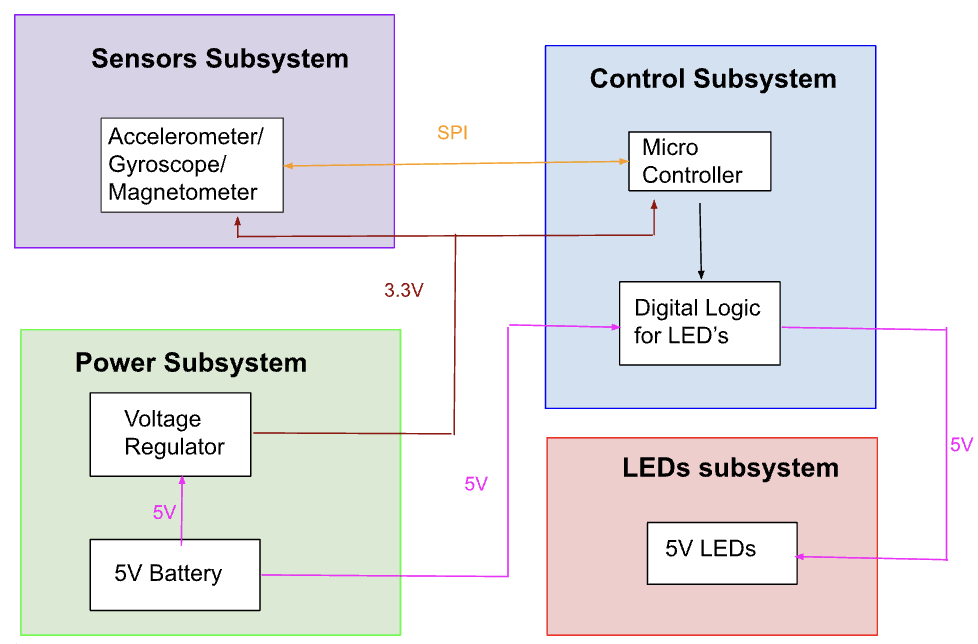
\includegraphics[width=0.8\textwidth]{block_diagram.png}
    \caption{Block Diagram of the system}
    \label{fig:my_label1}
\end{figure}
\subsection{Subsystem Overview}
    \subsubsection{Control Unit:} 
    We will design our PCB and microcontroller to be able to 
    receive data from the sensors, analyze the data, and display 
    the correct signal on the LEDs. The PCB will contain the 
    microcontroller, power the sensor suite, and contain digital 
    logic to control the LEDs. We will use the ESP32 microcontroller 
    to process the data from the sensors and output the correct 
    signals to the LEDs.
    \subsubsection{Power Subsystem:} 
	We will use a 5V rechargeable battery (Li-Ion or LiPo) to 
    power the components, 5V for the LEDs, and use a voltage 
    regulator to power the microcontroller and sensors at 3.3V. 
    We can place the battery in an inner pocket of the wearable,
     making it easy to wire it to all parts.
    \subsubsection{Sensors Subsystem:} 
    For the sensors, we will use a 3.3V 9dof IMU (accelerometer, 
    gyroscope, magnetometer) for each arm, and use the combined 
    data from both to determine the nature of the motion. In an 
    accident for example, the acceleration will spike, indicating 
    an accident. To distinguish between the other signals, we will
     use the gyroscope to determine the angle of the gesture. 
    \subsubsection{LEDs Subsystem:} 
    We will use 5V LED strips placed on the back and arms of the 
    wearable to display the information. The LEDs will be arranged 
    in a way that will make it clear to drivers and pedestrians
     what the rider is trying to signal.


\subsection{Subsystem Requirements}

\subsubsection{Control Unit:} 
The control unit should be able to receive SPI data from the 
sensor subsystem and use the ESP32 microcontroller to analyze 
it in order to route the 5V from the battery to power the LEDs. 

\textbf{Requirements:} The LEDs should light up according to the signals within 1 second.
Should also correctly identify the arm gestures with an accuracy of 90%

\subsubsection{Power Subsystem:} 
The Power subsystem should be able to output 5V through the control unit to power the LEDs, as well as output 3.3V to power the Control and Sensors subsystems. 

\textbf{Requirement:} The device should be able to last at least 1 hour on a full battery.

\subsubsection{Sensors Subsystem:}
The sensor subsystem should contain an IMU (accelerometer, gyroscope, and magnetometer) for each arm, read and controlled by the ESP32 microcontroller via an SPI signal. The data should contain acceleration, rotational, and cardinal direction data and should be filtered properly so as to not miss vital information and not cause false signals. The IMUs will be powered by a 3.3V input via the Power Subsystem.

\subsubsection{LEDs Subsystem:} 
The LED subsystem should be able to turn on the LEDs when powered by a 5V input from the control/power subsystems.

\textbf{Requirement:} The LEDs should be visible from a distance of at least 250 feet in low light conditions. 


\subsection{Tolerance Analysis}
The project will mainly depend on the signals received from the 
gyroscope and the accelerometer. Naturally, this will be our most 
important task. However, it might be tricky to set up the data to 
correctly reflect what we would like to receive. For instance, 
the acceleration would increase once the rider starts riding the 
bike, this might cause a false indication for turning the hazard 
lights on. The same might be true with slowing down. 

Additionally, we will use the gyroscope for handling the 
orientation of the hands to figure out the corresponding signals. 
We might face difficulties if the gyroscope is very sensitive to 
slight movements. Sometimes the rider would like to lift one hand 
slightly to shake it, that alone could cause a false turn signal. 

A big part of the process will be removing unnecessary information. 
In doing that, we take the risk of neglecting important data. 
If we set the acceleration threshold for the hazard too high, 
we might never turn the lights on when we actually need them. 

Lastly, we will be using many LEDs and a huge battery that allows 
recharging. We will need to be careful to not cause the battery to 
overheat. Overheating would run the risk of damaging the 
rider, as well as affecting the rest of the parts negatively. Our worst case operating temperature is 77.8 degrees 
celsius, but will likely never reach this because we will not 
be using the wifi modem in the ESP32 controller, greatly reducing 
the current draw. 

\section{Ethics and Safety}
\subsection{Ethical Considerations}
We must consider privacy concerns of the user because we will 
be collecting and processing data constantly during a 
ride/commute. We can limit the data collection to IMU data, 
so that nothing personally identifiable is collected, as well 
as deleting any data past a certain period of time. We also
have to consider the accuracy of the system, as it is a safety
device. We have to make sure that the system is reliable and
accurate, so that it does not fail when it is needed most.
We also have to consider the patent and intellectual property
rights of the system.

\subsection{Safety Considerations}
We have to consider the brightness of the LEDs, and 
if they can be distracting to other drivers and pedestrians. 
Having bright LEDs can be beneficial for low light or adverse 
conditions, but can also be harmful if they dazzle other drivers, 
impairing their vision. There are also consumer product safety 
standards that we need to follow for wearable technology, such 
as those related to electronics devices and battery safety.



% \begin{thebibliography}{99}
% %\bibitem{5} A. Mandelis, ``\emph{Diffusion waves and their uses}", Phys. Today \textbf{66}, 29-34 (2000).

% \end{thebibliography}


\end{document} 